\begin{figure*}[t]
\centering
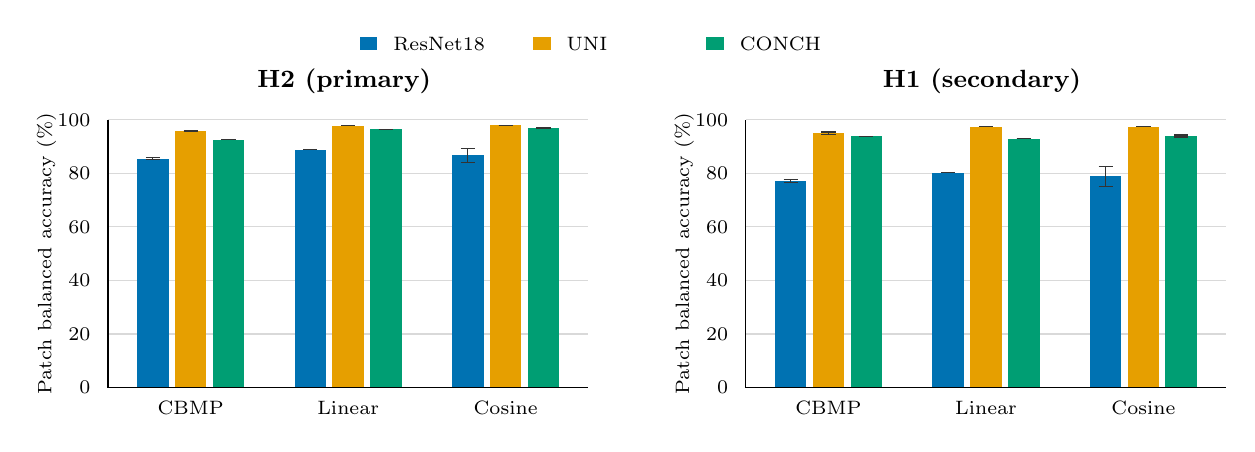
\begin{tikzpicture}[font=\scriptsize,y=.85cm]
\definecolor{pathologyResnetBlue}{HTML}{0072B2}
\definecolor{pathologyUniOrange}{HTML}{E69F00}
\definecolor{pathologyConchGreen}{HTML}{009E73}
\fill[pathologyResnetBlue] (4.10,5.05) rectangle (4.32,5.23);
\node[anchor=west] at (4.40,5.14) {ResNet18};
\fill[pathologyUniOrange] (6.30,5.05) rectangle (6.52,5.23);
\node[anchor=west] at (6.60,5.14) {UNI};
\fill[pathologyConchGreen] (8.50,5.05) rectangle (8.72,5.23);
\node[anchor=west] at (8.80,5.14) {CONCH};
\begin{scope}[xshift=0.00cm]
\node[font=\small\bfseries] at (3.9,4.58) {H2 (primary)};
\draw[black!15] (.9,0.000) -- (7.0,0.000);
\node[anchor=east] at (.8,0.000) {0};
\draw[black!15] (.9,0.800) -- (7.0,0.800);
\node[anchor=east] at (.8,0.800) {20};
\draw[black!15] (.9,1.600) -- (7.0,1.600);
\node[anchor=east] at (.8,1.600) {40};
\draw[black!15] (.9,2.400) -- (7.0,2.400);
\node[anchor=east] at (.8,2.400) {60};
\draw[black!15] (.9,3.200) -- (7.0,3.200);
\node[anchor=east] at (.8,3.200) {80};
\draw[black!15] (.9,4.000) -- (7.0,4.000);
\node[anchor=east] at (.8,4.000) {100};
\node[rotate=90] at (.12,2) {Patch balanced accuracy (\%)};
\fill[pathologyResnetBlue] (1.270,0) rectangle (1.670,3.42177);
\draw[black!80] (1.470,3.40883) -- (1.470,3.43471);
\draw[black!80] (1.380,3.40883) -- (1.560,3.40883);
\draw[black!80] (1.380,3.43471) -- (1.560,3.43471);
\fill[pathologyUniOrange] (1.750,0) rectangle (2.150,3.83201);
\draw[black!80] (1.950,3.82532) -- (1.950,3.83870);
\draw[black!80] (1.860,3.82532) -- (2.040,3.82532);
\draw[black!80] (1.860,3.83870) -- (2.040,3.83870);
\fill[pathologyConchGreen] (2.230,0) rectangle (2.630,3.70531);
\draw[black!80] (2.430,3.70531) -- (2.430,3.70531);
\draw[black!80] (2.340,3.70531) -- (2.520,3.70531);
\draw[black!80] (2.340,3.70531) -- (2.520,3.70531);
\node at (1.950,-.30) {CBMP};
\fill[pathologyResnetBlue] (3.270,0) rectangle (3.670,3.55539);
\draw[black!80] (3.470,3.55539) -- (3.470,3.55539);
\draw[black!80] (3.380,3.55539) -- (3.560,3.55539);
\draw[black!80] (3.380,3.55539) -- (3.560,3.55539);
\fill[pathologyUniOrange] (3.750,0) rectangle (4.150,3.90870);
\draw[black!80] (3.950,3.90870) -- (3.950,3.90870);
\draw[black!80] (3.860,3.90870) -- (4.040,3.90870);
\draw[black!80] (3.860,3.90870) -- (4.040,3.90870);
\fill[pathologyConchGreen] (4.230,0) rectangle (4.630,3.85998);
\draw[black!80] (4.430,3.85998) -- (4.430,3.85998);
\draw[black!80] (4.340,3.85998) -- (4.520,3.85998);
\draw[black!80] (4.340,3.85998) -- (4.520,3.85998);
\node at (3.950,-.30) {Linear};
\fill[pathologyResnetBlue] (5.270,0) rectangle (5.670,3.46901);
\draw[black!80] (5.470,3.36855) -- (5.470,3.56947);
\draw[black!80] (5.380,3.36855) -- (5.560,3.36855);
\draw[black!80] (5.380,3.56947) -- (5.560,3.56947);
\fill[pathologyUniOrange] (5.750,0) rectangle (6.150,3.91825);
\draw[black!80] (5.950,3.91540) -- (5.950,3.92109);
\draw[black!80] (5.860,3.91540) -- (6.040,3.91540);
\draw[black!80] (5.860,3.92109) -- (6.040,3.92109);
\fill[pathologyConchGreen] (6.230,0) rectangle (6.630,3.87516);
\draw[black!80] (6.430,3.87257) -- (6.430,3.87775);
\draw[black!80] (6.340,3.87257) -- (6.520,3.87257);
\draw[black!80] (6.340,3.87775) -- (6.520,3.87775);
\node at (5.950,-.30) {Cosine};
\draw (.9,0) -- (7,0);
\draw (.9,0) -- (.9,4);
\end{scope}
\begin{scope}[xshift=8.10cm]
\node[font=\small\bfseries] at (3.9,4.58) {H1 (secondary)};
\draw[black!15] (.9,0.000) -- (7.0,0.000);
\node[anchor=east] at (.8,0.000) {0};
\draw[black!15] (.9,0.800) -- (7.0,0.800);
\node[anchor=east] at (.8,0.800) {20};
\draw[black!15] (.9,1.600) -- (7.0,1.600);
\node[anchor=east] at (.8,1.600) {40};
\draw[black!15] (.9,2.400) -- (7.0,2.400);
\node[anchor=east] at (.8,2.400) {60};
\draw[black!15] (.9,3.200) -- (7.0,3.200);
\node[anchor=east] at (.8,3.200) {80};
\draw[black!15] (.9,4.000) -- (7.0,4.000);
\node[anchor=east] at (.8,4.000) {100};
\node[rotate=90] at (.12,2) {Patch balanced accuracy (\%)};
\fill[pathologyResnetBlue] (1.270,0) rectangle (1.670,3.08576);
\draw[black!80] (1.470,3.06349) -- (1.470,3.10802);
\draw[black!80] (1.380,3.06349) -- (1.560,3.06349);
\draw[black!80] (1.380,3.10802) -- (1.560,3.10802);
\fill[pathologyUniOrange] (1.750,0) rectangle (2.150,3.80071);
\draw[black!80] (1.950,3.78366) -- (1.950,3.81776);
\draw[black!80] (1.860,3.78366) -- (2.040,3.78366);
\draw[black!80] (1.860,3.81776) -- (2.040,3.81776);
\fill[pathologyConchGreen] (2.230,0) rectangle (2.630,3.75163);
\draw[black!80] (2.430,3.75163) -- (2.430,3.75163);
\draw[black!80] (2.340,3.75163) -- (2.520,3.75163);
\draw[black!80] (2.340,3.75163) -- (2.520,3.75163);
\node at (1.950,-.30) {CBMP};
\fill[pathologyResnetBlue] (3.270,0) rectangle (3.670,3.21201);
\draw[black!80] (3.470,3.21201) -- (3.470,3.21201);
\draw[black!80] (3.380,3.21201) -- (3.560,3.21201);
\draw[black!80] (3.380,3.21201) -- (3.560,3.21201);
\fill[pathologyUniOrange] (3.750,0) rectangle (4.150,3.89895);
\draw[black!80] (3.950,3.89895) -- (3.950,3.89895);
\draw[black!80] (3.860,3.89895) -- (4.040,3.89895);
\draw[black!80] (3.860,3.89895) -- (4.040,3.89895);
\fill[pathologyConchGreen] (4.230,0) rectangle (4.630,3.71525);
\draw[black!80] (4.430,3.71525) -- (4.430,3.71525);
\draw[black!80] (4.340,3.71525) -- (4.520,3.71525);
\draw[black!80] (4.340,3.71525) -- (4.520,3.71525);
\node at (3.950,-.30) {Linear};
\fill[pathologyResnetBlue] (5.270,0) rectangle (5.670,3.15606);
\draw[black!80] (5.470,3.00466) -- (5.470,3.30745);
\draw[black!80] (5.380,3.00466) -- (5.560,3.00466);
\draw[black!80] (5.380,3.30745) -- (5.560,3.30745);
\fill[pathologyUniOrange] (5.750,0) rectangle (6.150,3.89918);
\draw[black!80] (5.950,3.89708) -- (5.950,3.90129);
\draw[black!80] (5.860,3.89708) -- (6.040,3.89708);
\draw[black!80] (5.860,3.90129) -- (6.040,3.90129);
\fill[pathologyConchGreen] (6.230,0) rectangle (6.630,3.75816);
\draw[black!80] (6.430,3.74296) -- (6.430,3.77335);
\draw[black!80] (6.340,3.74296) -- (6.520,3.74296);
\draw[black!80] (6.340,3.77335) -- (6.520,3.77335);
\node at (5.950,-.30) {Cosine};
\draw (.9,0) -- (7,0);
\draw (.9,0) -- (.9,4);
\end{scope}
\end{tikzpicture}
\caption{Patch-level balanced accuracy on the identical custom CAMELYON subset under four-candidate source-only selection. Bars show ten-seed means; whiskers show fitting-seed standard deviation, not patient- or hospital-population uncertainty. CBMP, linear logistic and trained cosine are prespecified views; all nine heads appear in the accompanying tables.}
\label{fig:pathology_encoders_patch}
\end{figure*}
